\section{Backend Implementation}
\subsection{Introduction}
The backend of the Intern Management Platform is built on Drupal 10, using VOID Agency's Vactory distribution. We chose this stack for its modularity and JSON:API support, which enables seamless frontend integration. The backend consists of three main components: the Main Website, Candidate Space, and custom modules for recruitment automation.

\subsection{Drupal Architecture and API Strategy}

\subsubsection{What is Drupal?}
Drupal is an open-source content management system (CMS) used to build and manage websites. It provides a flexible back office for content creation, user management, and site configuration.

\subsubsection{Our Use of Drupal}
In our project, we use Drupal mainly as a backend service. The Drupal back office is used for content management, while the frontend is built separately. We do not use Drupal's default theming or page rendering for the public site.

\subsubsection{Exposing Content with JSON:API}
To connect Drupal with our frontend, we enabled and configured the \textbf{JSON:API} module. This module allows us to expose Drupal content, users, menus, and other entities as RESTful API endpoints. These endpoints are configurable and can be consumed directly by the frontend application.

\begin{figure}[H]
    \centering
    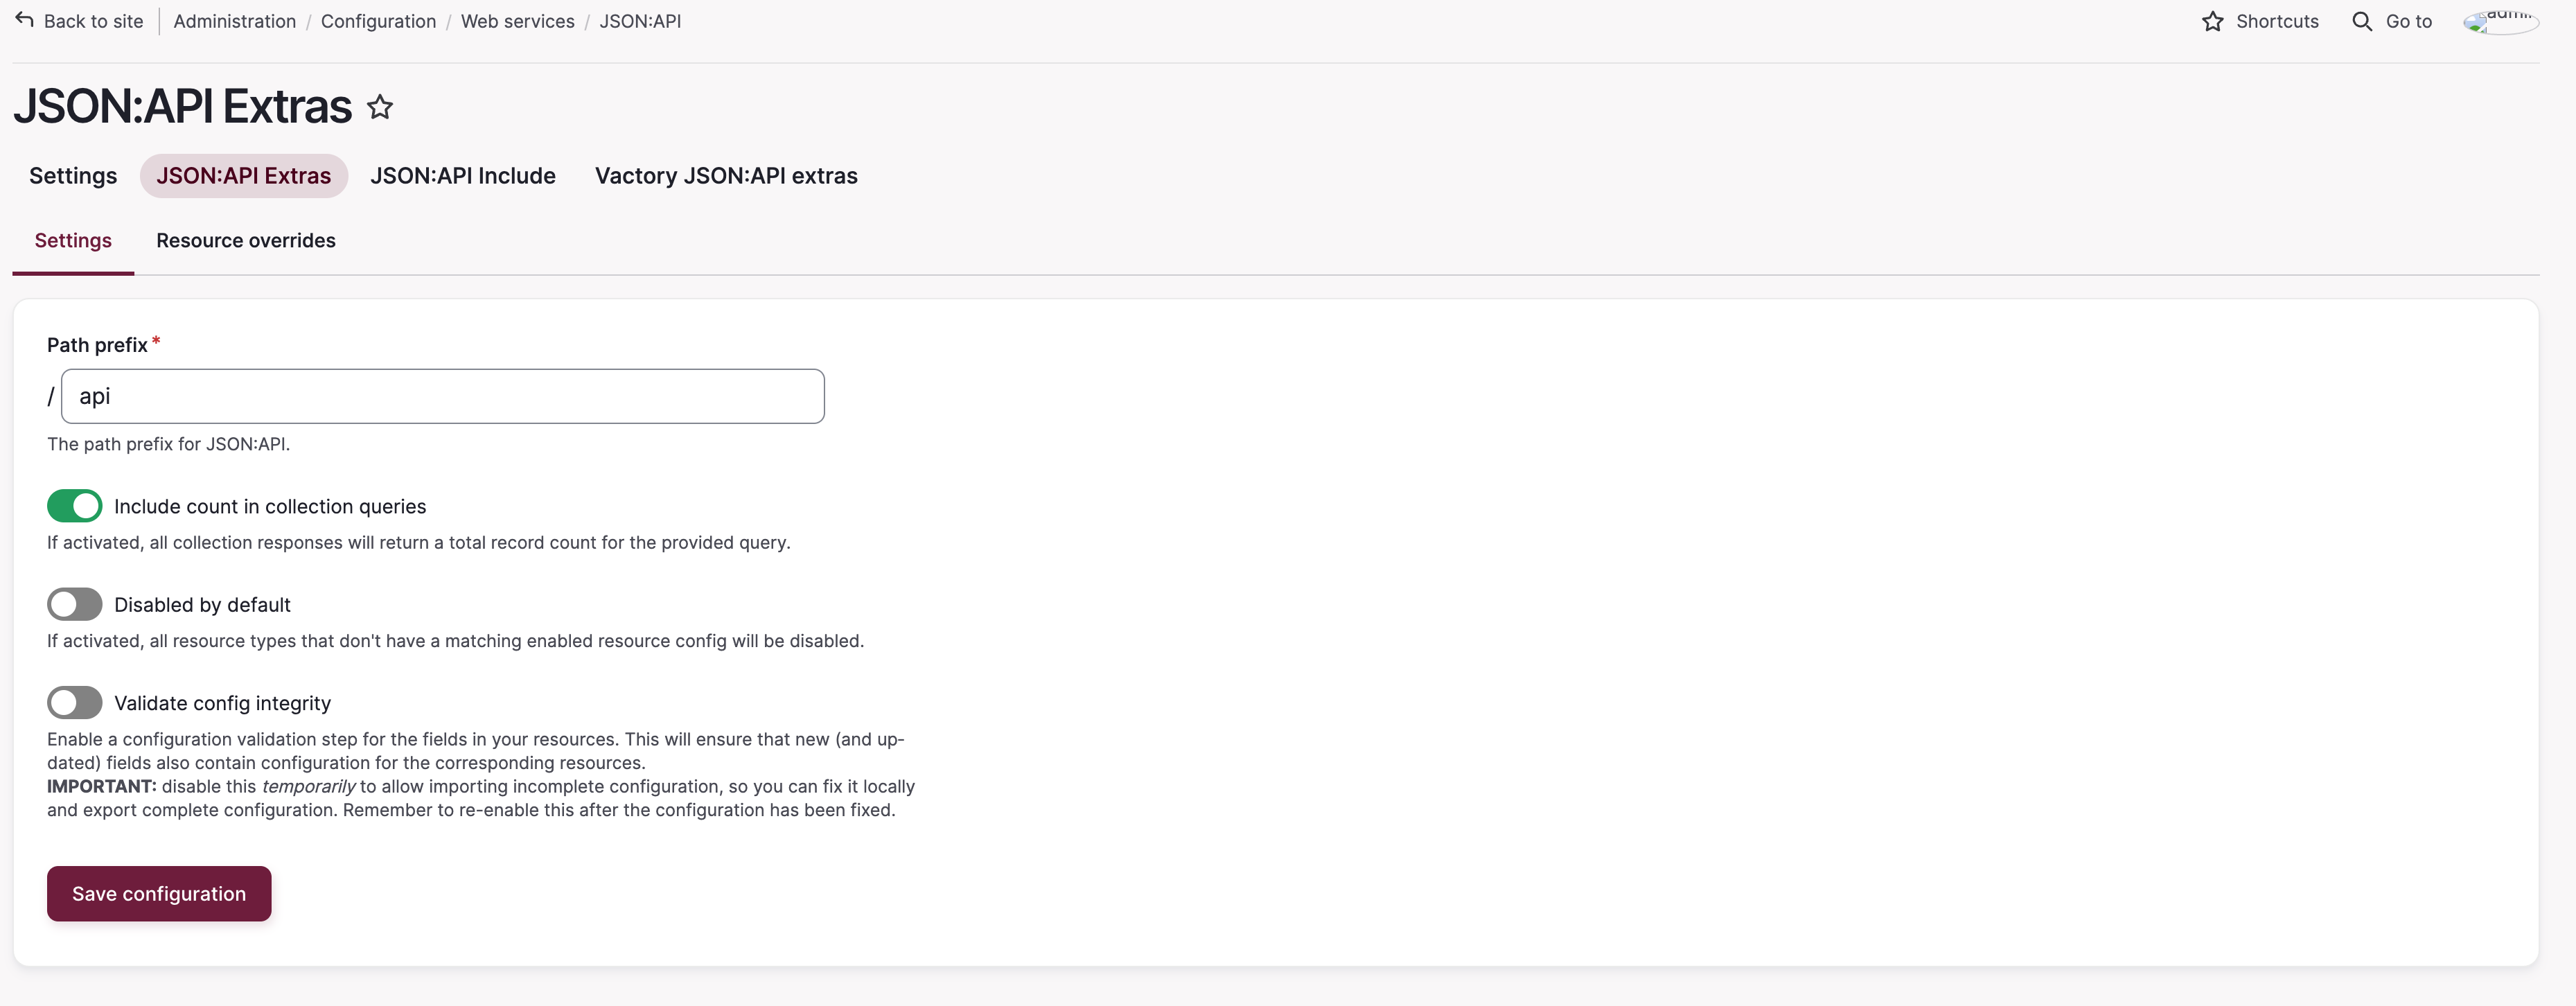
\includegraphics[width=0.8\textwidth]{images/json-api-path-configuration.png}
    \caption{JSON:API endpoint configuration with path prefix /api}
    \label{fig:jsonapi_path_config}
\end{figure}

\begin{figure}[H]
    \centering
    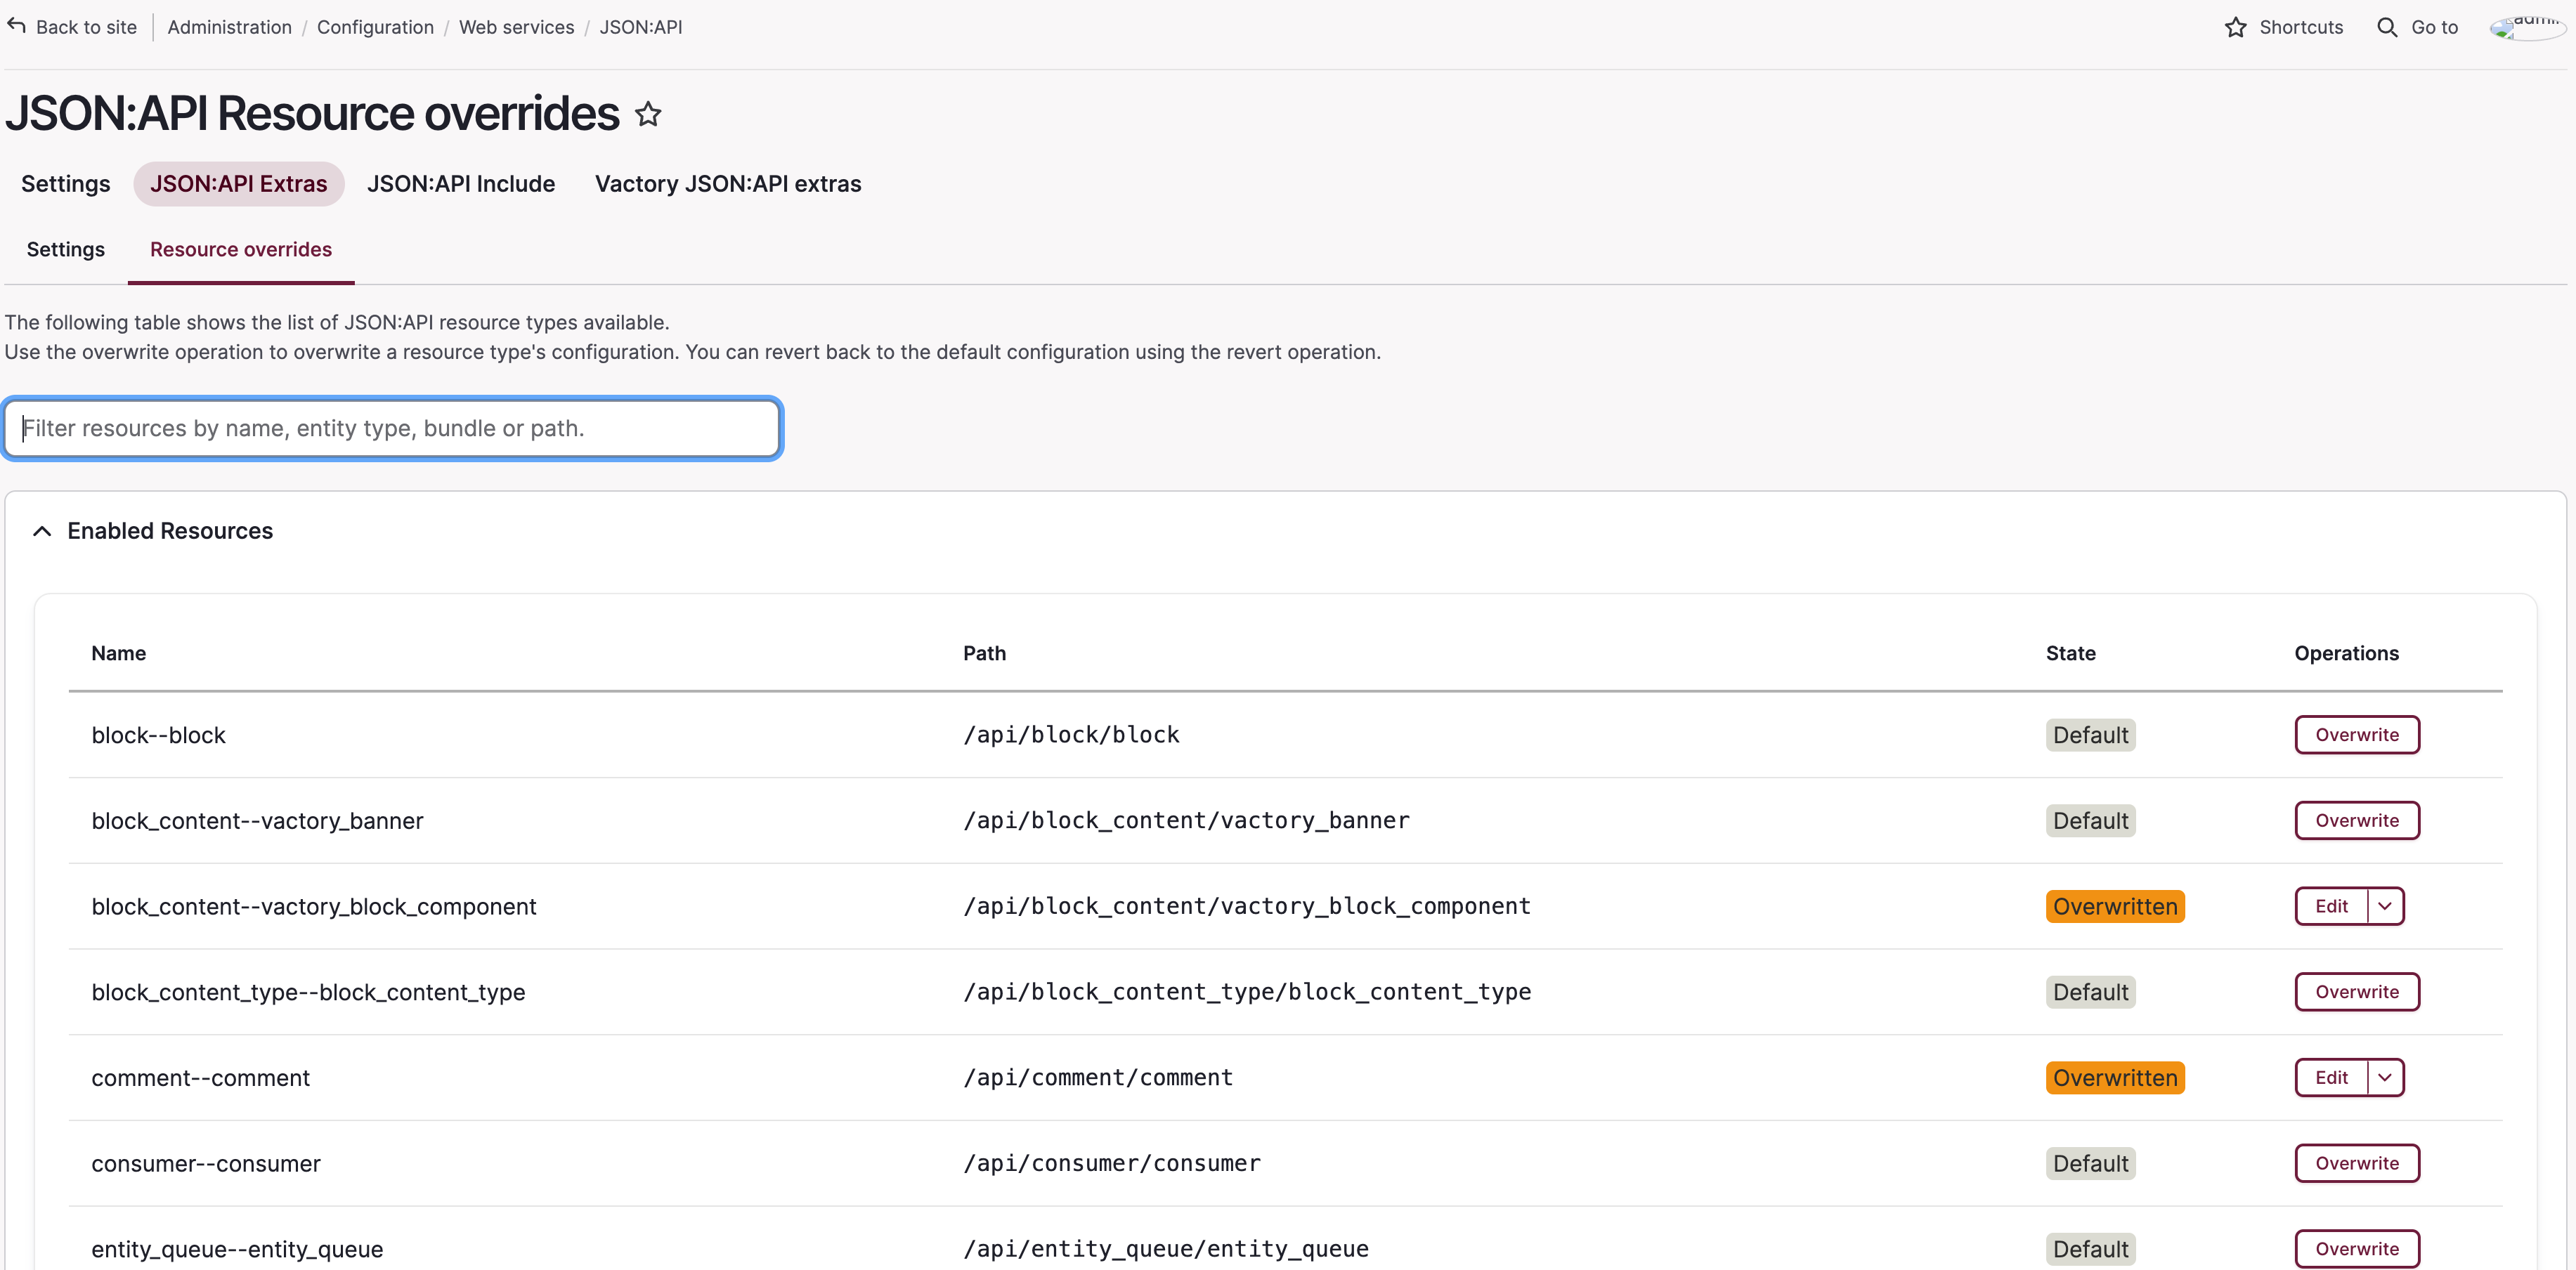
\includegraphics[width=0.9\textwidth]{images/json-api-recources.png}
    \caption{Exposed JSON:API resources in Drupal}
    \label{fig:jsonapi_resources}
\end{figure}

\subsubsection{Custom API Endpoints for Menus and Translations}
For essential features like menus and translations, we configured two custom API endpoints:
\begin{itemize}
    \item \texttt{/api/\_translations} — Returns translation data for the site.
    \item \texttt{/api/\_menus?menu\_name=\{main,footer,...\}} — Returns menu structures for navigation.
\end{itemize}

\subsubsection{Building Website Structure with Dynamic Fields}
To enable flexible page construction, we use the \textbf{Dynamic Field} module and a modular development approach. Website components—such as headers, footers, and card lists—are implemented as reusable Drupal entities, which we refer to as \textit{widgets}. These widgets are defined in the codebase and can be placed visually within page layouts using the Drupal back office.

The typical workflow is as follows:
\begin{enumerate}
    \item Create widget templates in the codebase, specifying the data to be exposed.
    \item Use the Drupal interface to assign widgets to specific page regions.
    \item The JSON:API module automatically exposes the page structure and widget data as API endpoints.
    \item Consume these endpoints to render the final user interface.
\end{enumerate}

\begin{figure}[H]
    \centering
    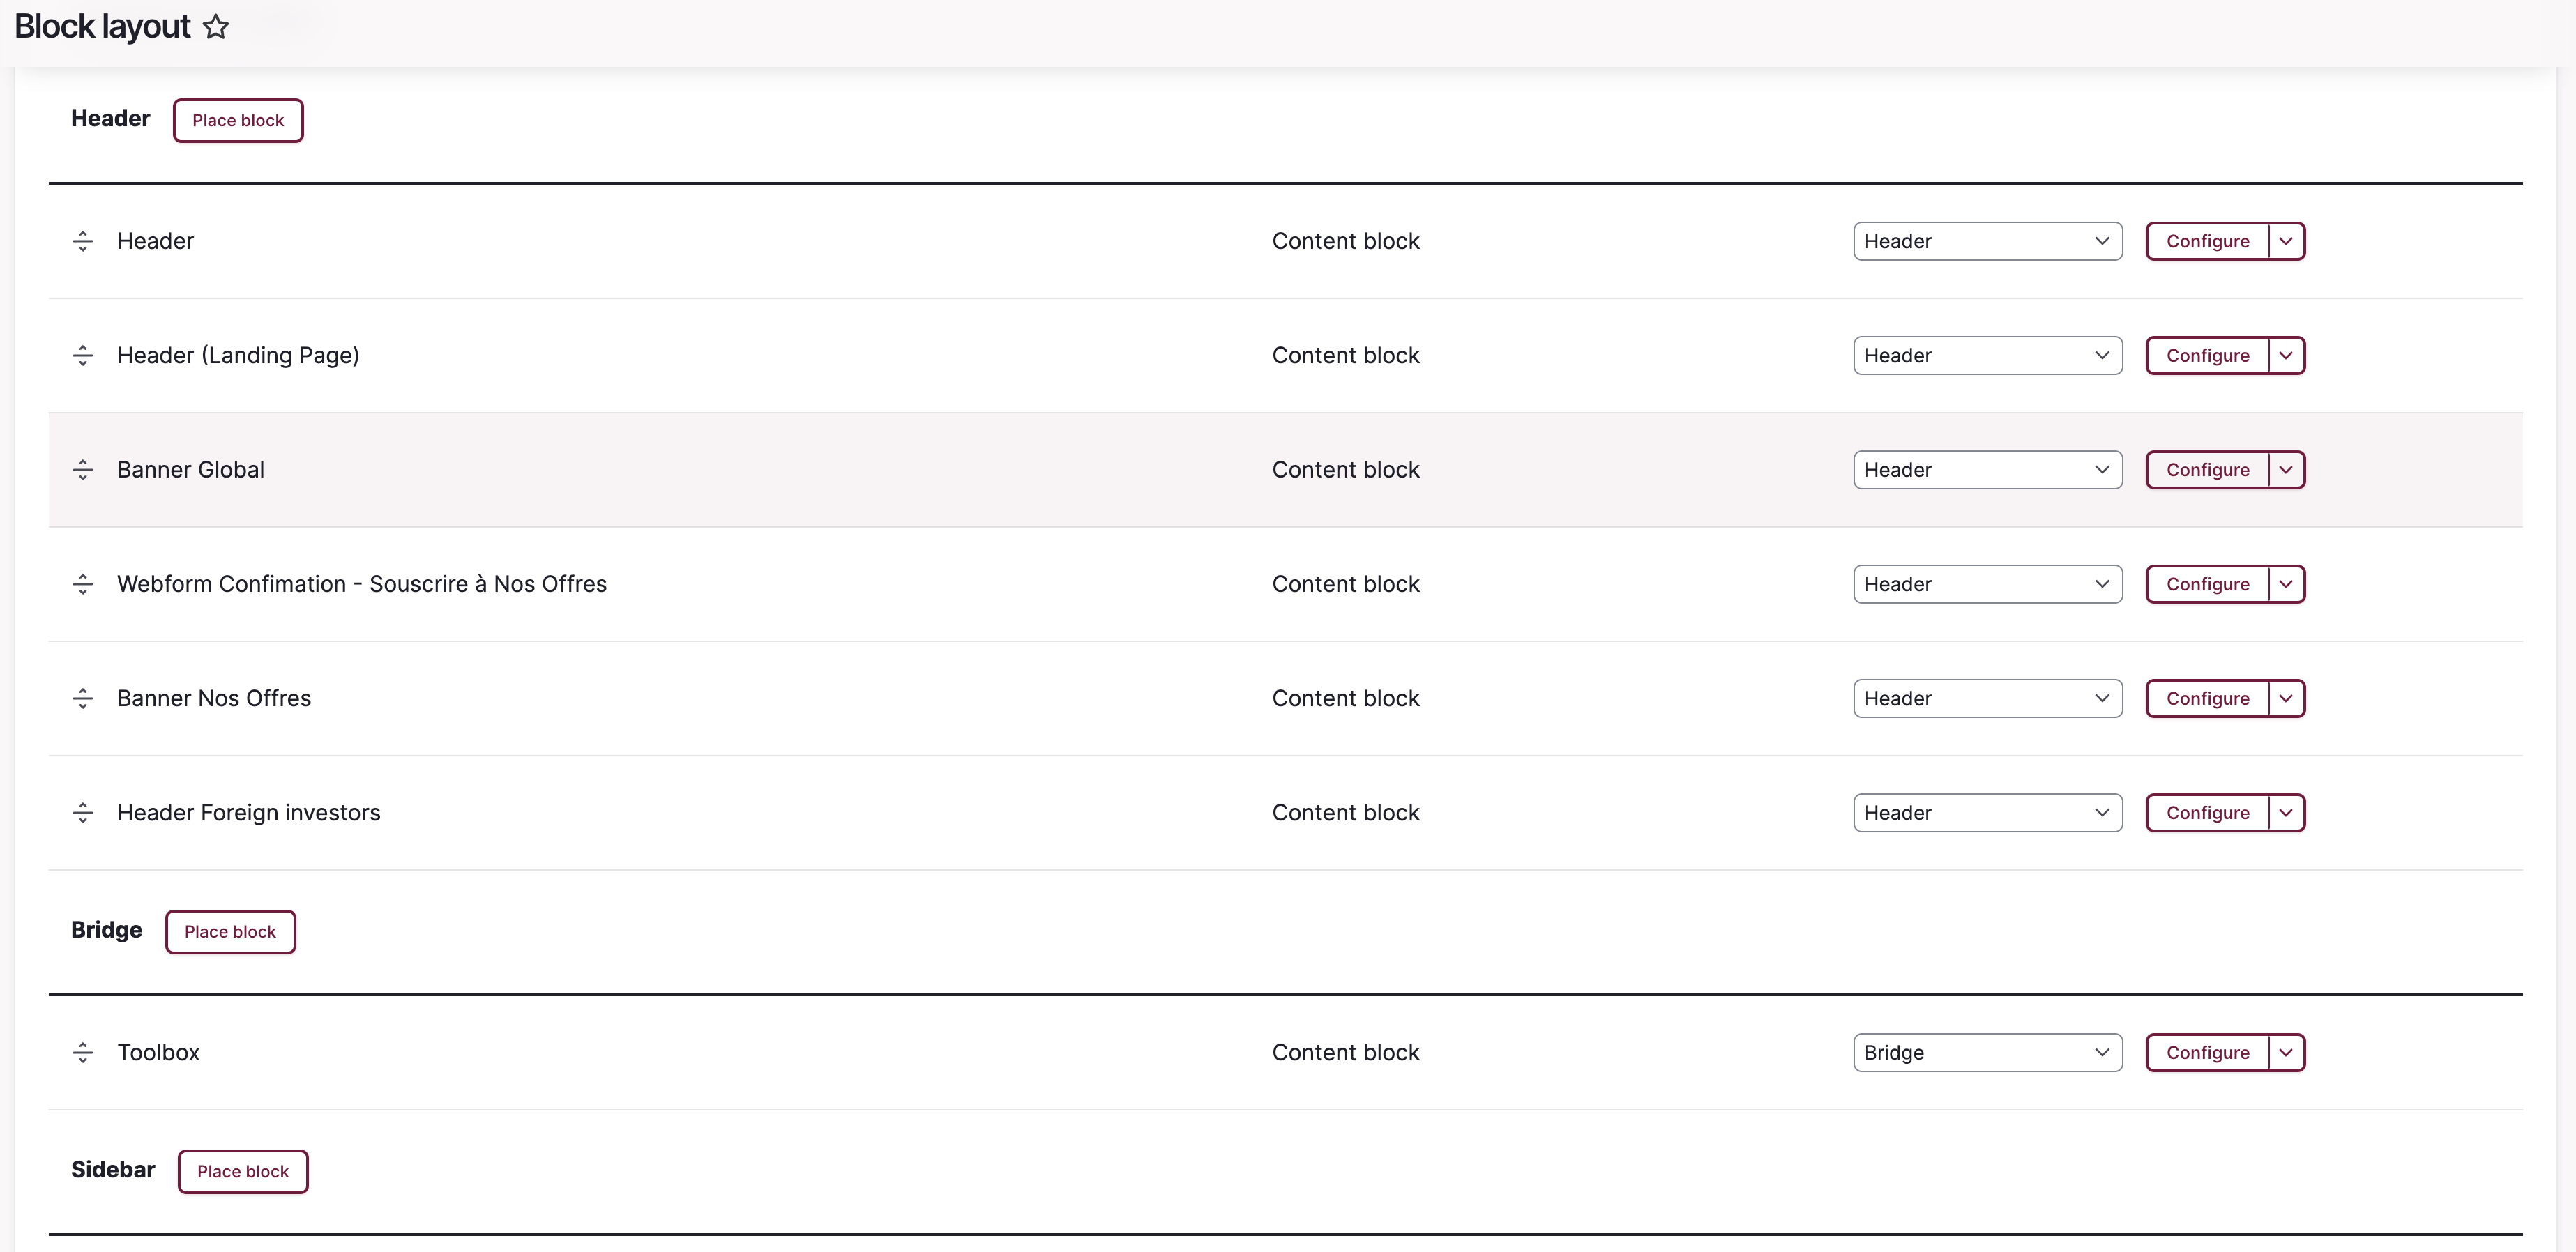
\includegraphics[width=0.95\textwidth]{images/structuring-page-BO.png}
    \caption{Visual placement of widgets (blocks) in the Drupal back office}
    \label{fig:drupal_block_layout}
\end{figure}

This decoupled approach allows for rapid content updates and consistent data delivery to the frontend, while maintaining a clear separation between content management and presentation.

% \subsubsection{Example: Dynamic Field Implementation}
% We will provide a practical example showing how a dynamic field is implemented, from backend entity definition to its exposure via the API and consumption on the frontend.

% (You can insert your example here.)



\subsection{Performance Optimization with Memcached}
To enhance backend response time and reduce database load, we implemented Memcached as our caching solution. In our Docker-based architecture, Memcached runs as a dedicated container, communicating directly with Drupal through our internal Docker network.

Memcached improves our platform's performance by:
\begin{itemize}
    \item Caching frequently accessed data in memory (entities, views, routes)
    \item Reducing database queries and disk I/O operations
    \item Providing near-instant access to cached content
    \item Enabling horizontal scaling of the caching layer
\end{itemize}

This caching strategy is particularly effective for our recruitment platform, where multiple users frequently access the same content like job listings and candidate profiles. During peak recruitment periods, Memcached helps maintain fast response times even under high traffic loads.
\begin{figure}[H]
  \centering
  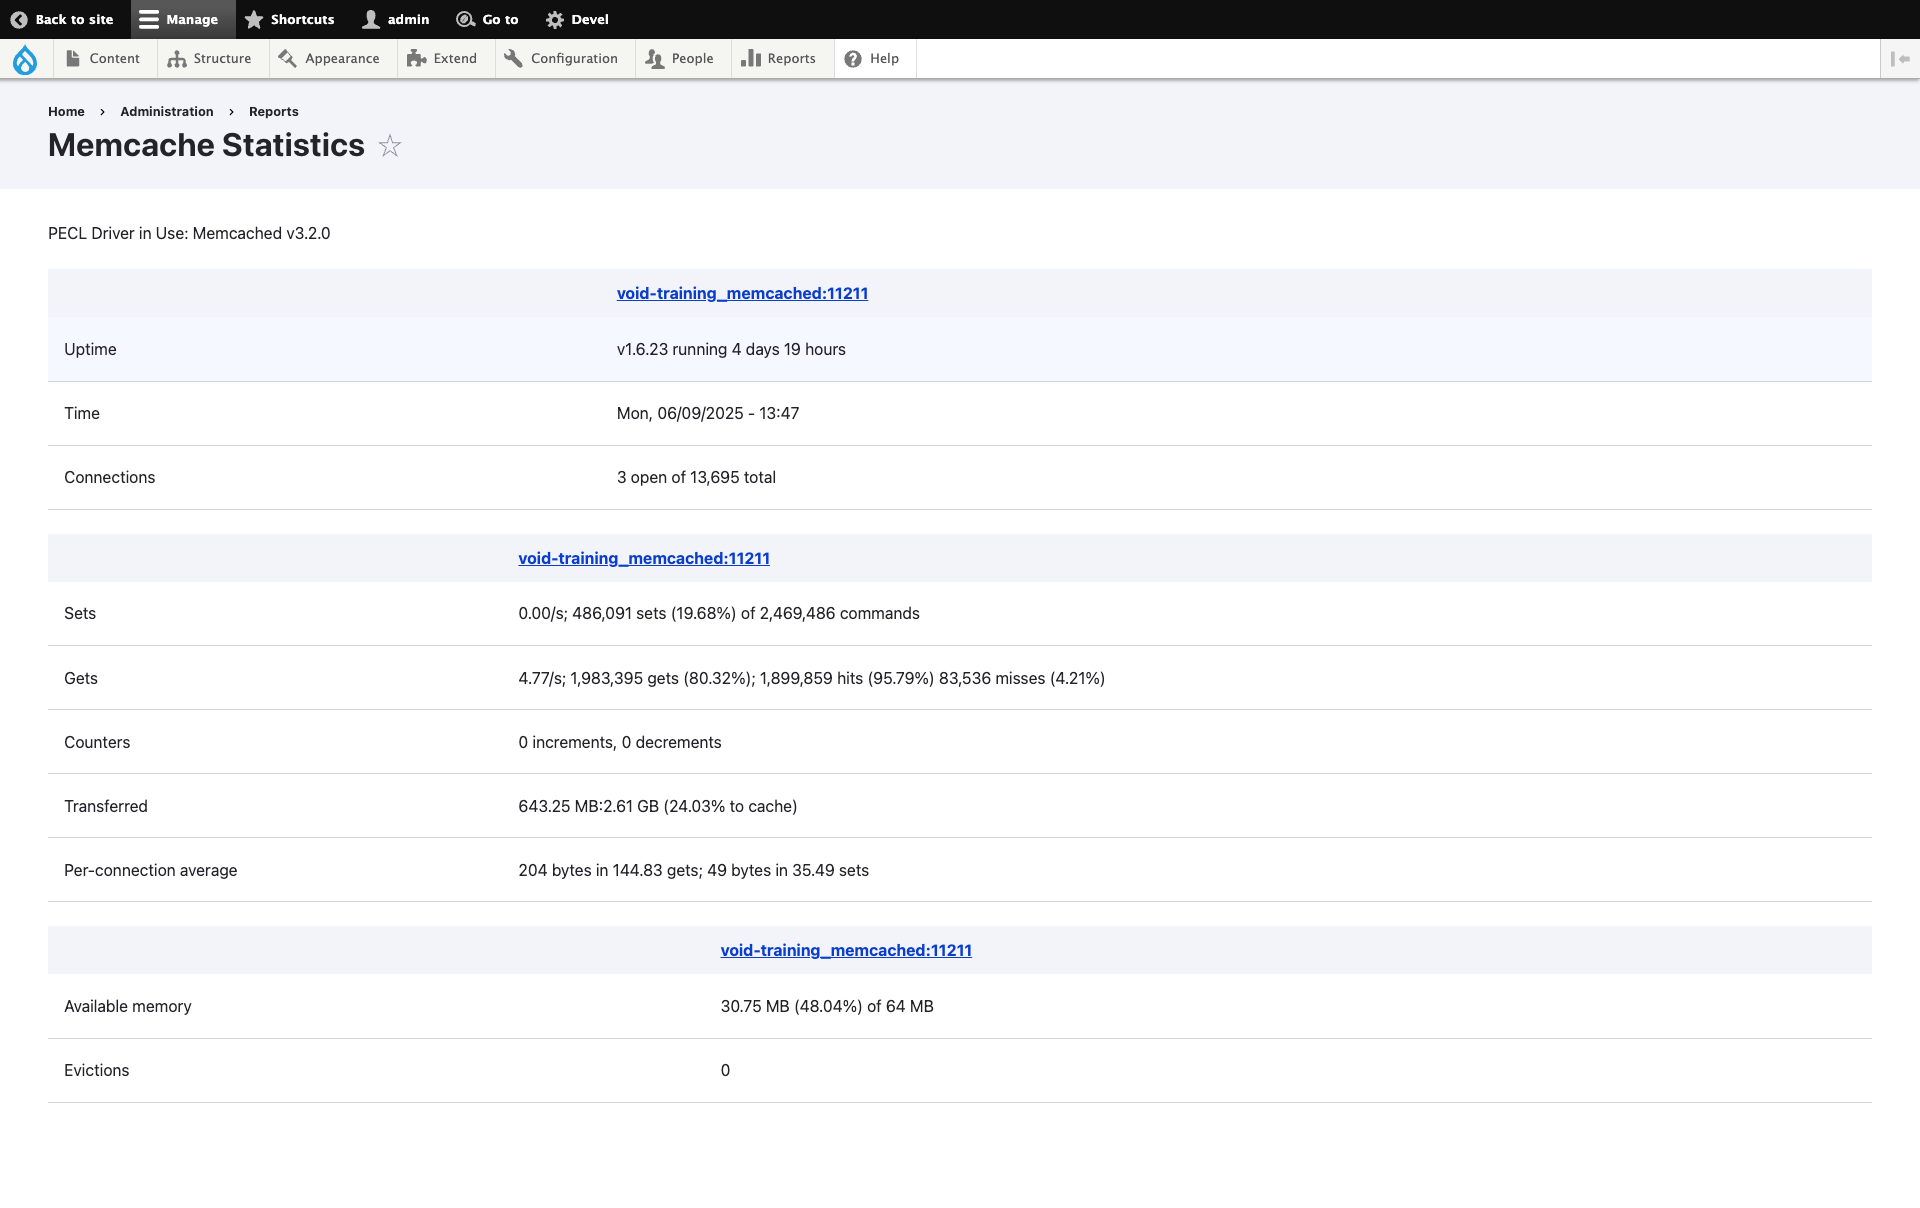
\includegraphics[width=\textwidth]{images/memcached_ui.png}
  \caption{Memcached UI}
  \label{fig:memcached}
\end{figure}

\subsection{Email Debugging with MailHog}
We use MailHog as a Docker container for email testing in development. It provides a web interface at port 8025 for viewing emails and an SMTP server at port 1025 for intercepting outgoing messages.

Drupal is configured to use MailHog's SMTP server through the Symfony Mailer module, which handles all system emails including account notifications, interview scheduling, evaluation reports, and password resets. This containerized setup ensures consistent email testing across all development environments.

\subsection{Widget System Architecture and Discovery Process}
\noindent
The backbone of our content management strategy relies on Vactory's widget system, which implements dynamic, reusable content components that bridge backend configuration with frontend rendering. Understanding the widget lifecycle reveals how Drupal automatically discovers, categorizes, and exposes these components to content editors.

\medskip

\noindent
The widget discovery process follows a structured technical workflow:

\begin{enumerate}
    \item \textbf{Widget Definition}: Each widget consists of a directory containing a \texttt{settings.yml} file that defines metadata, JSON:API queries, field structures, and categorization information. This YAML configuration acts as the widget's blueprint, specifying data sources, field types, and display preferences.
    
    \item \textbf{Automatic Discovery}: During Drupal's module discovery phase, the system scans all enabled modules for widget directories. The presence of a \texttt{settings.yml} file signals to Drupal that the directory contains a valid widget definition.
    
    \item \textbf{Plugin Registration}: Drupal's plugin system registers each discovered widget as a paragraph type, making it available through the administrative interface. The widget's metadata from the YAML file determines its category, id, and content.
    
    \item \textbf{Frontend Mapping}: A corresponding Webpack plugin on the frontend side scans for widget files matching specific patterns (\texttt{*Widget.jsx}). This plugin extracts configuration IDs from each React component and generates a mapping file that links backend widget IDs to their frontend implementations.
    
    \item \textbf{Template Selection Interface}: Content editors access widgets through Drupal's paragraph interface, where widgets are organized by categories (Academy, Banners, Content, Void Training, etc.). This categorization is defined in each widget's YAML configuration.
\end{enumerate}

\medskip

\noindent
When content editors create or edit pages, they encounter a streamlined widget selection process. The template chooser displays widgets organized by functional categories, allowing editors to quickly locate appropriate components for their content needs.

\begin{figure}[H]
    \centering
    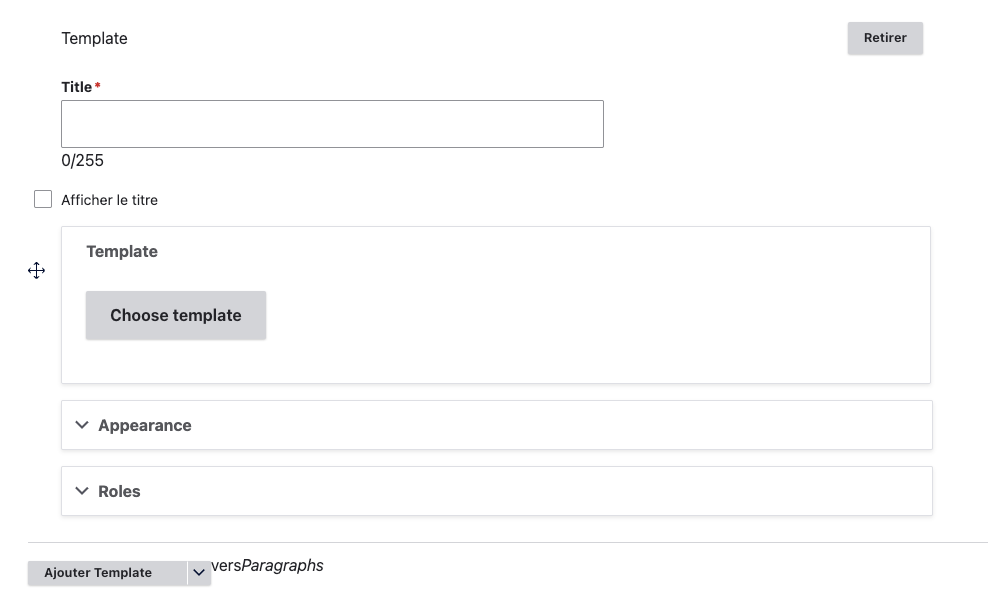
\includegraphics[width=\textwidth]{images/widget_selection.png}
    \caption{Widget Selection Interface with Category Tabs}
    \label{fig:widget_selection}
\end{figure}

\noindent
Within each category, editors can browse available widget templates. For the Void Training project, custom widgets were developed specifically for recruitment and training content, including process flows, call-to-action sections, and testimonial displays.

\begin{figure}[H]
    \centering
    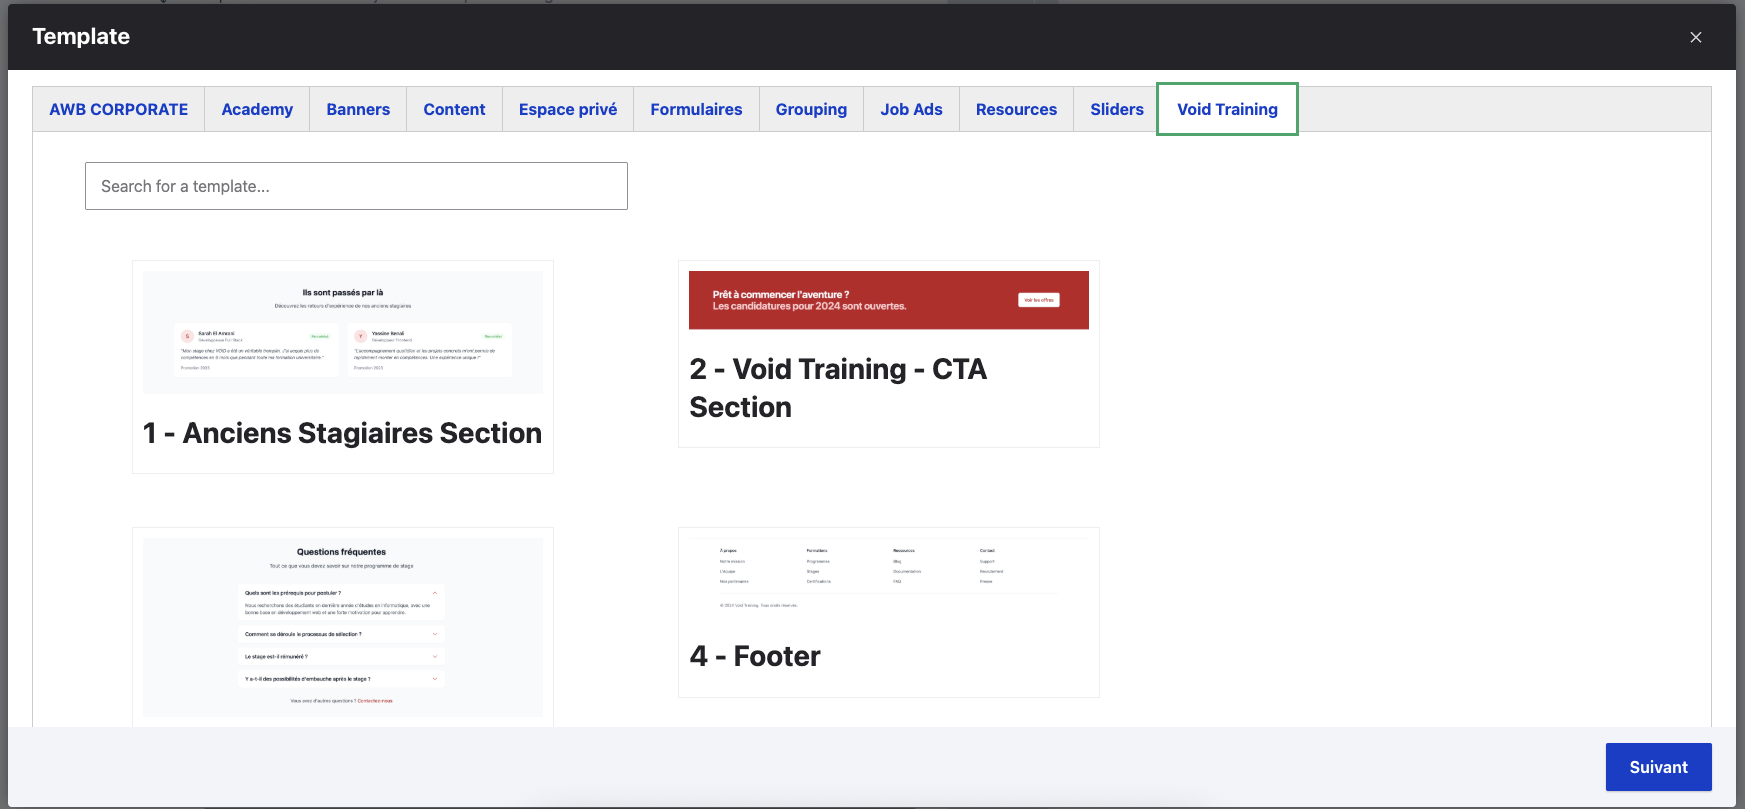
\includegraphics[width=\textwidth]{images/widget_lists.png}
    \caption{Available Widget Templates in Void Training Category}
    \label{fig:widget_lists}
\end{figure}

\noindent
Once a widget is selected, editors access a dynamic configuration interface. Each widget exposes different field types and structures based on its YAML definition. For complex widgets like the Recruitment Process widget, editors can configure multiple components, titles, descriptions, and process steps through an intuitive form interface.

\begin{figure}[H]
    \centering
    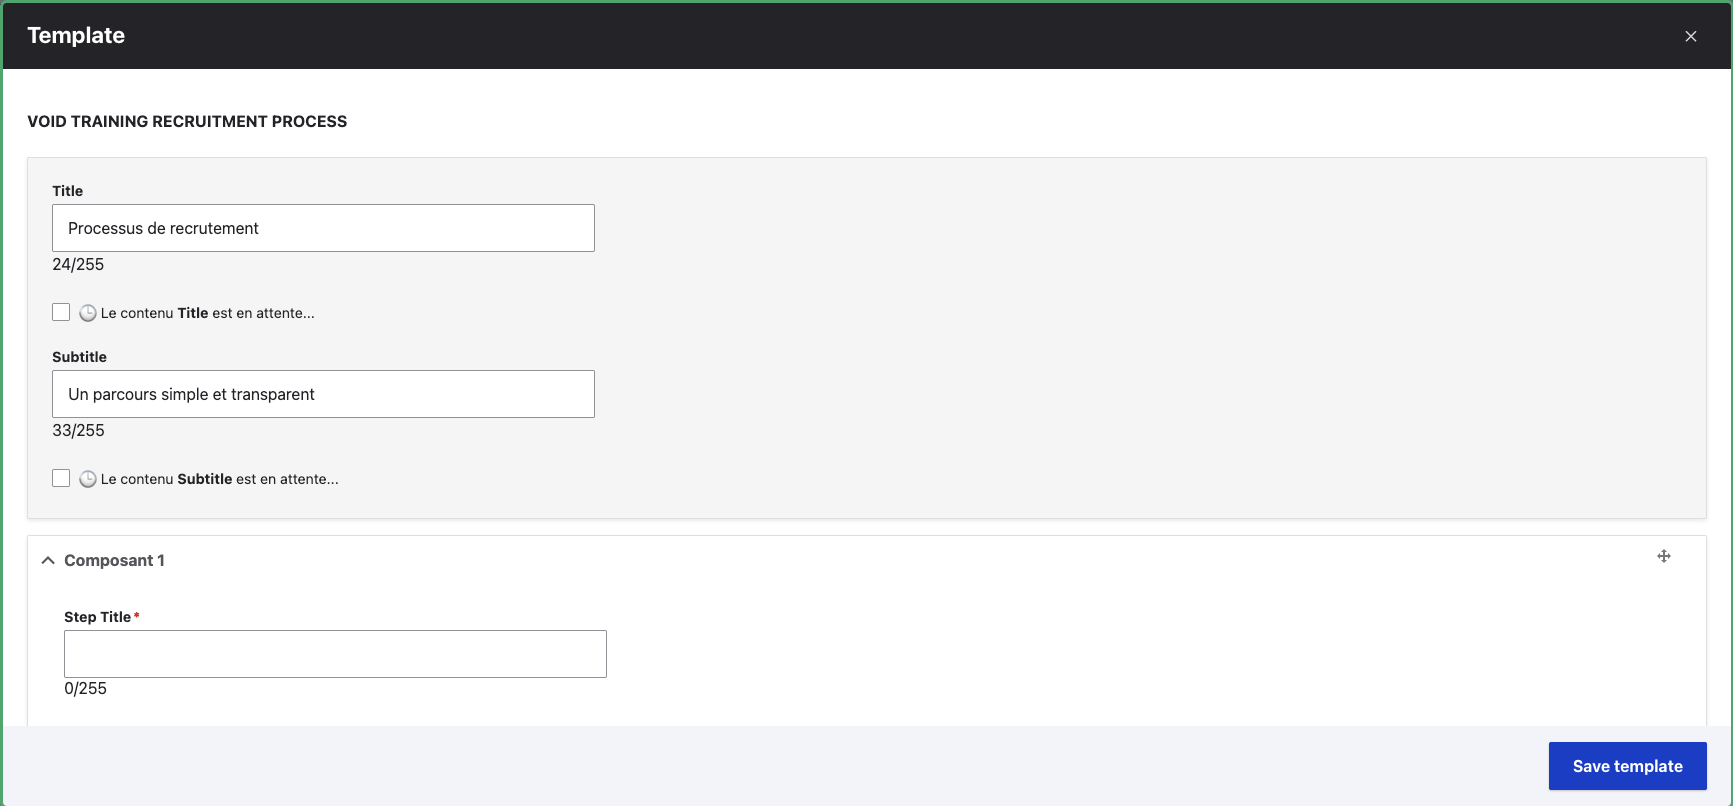
\includegraphics[width=\textwidth]{images/widget_content.png}
    \caption{Widget Configuration Interface for Recruitment Process}
    \label{fig:widget_content}
\end{figure}


\subsection{Main Website Backend Structure}
The main website's backend is built using a widget-based architecture, where each widget is a Drupal paragraph type that can be configured and reused across the site. These widgets are exposed through JSON:API for frontend consumption, making them easily accessible and maintainable.

The platform includes two main categories of widgets: Core Layout Widgets and Content Display Widgets. Core Layout Widgets handle the fundamental structure of the site. The Header Widget manages navigation and user authentication, while the Footer Widget provides company information and quick links. The Hero Widget creates engaging landing sections with customizable backgrounds and call-to-action elements.

Content Display Widgets focus on presenting information in various formats. Card Listing Widgets offer three variations: Tagged Cards for filtered content, Duration Cards for time-based content, and Numbered Cards for sequential information. The Testimonial Widget displays user feedback with ratings and profile information, while the Slider Widget creates dynamic content carousels with responsive controls.

A key feature is the Project Showcase Widget, which displays intern projects with details like technologies used, duration, and links to repositories. All widgets are designed to be fully configurable through the Drupal interface, responsive across devices, and consistent in their styling and behavior.

This widget-based approach allows content editors to create engaging layouts without technical intervention while maintaining a consistent presentation across the site.

% \subsection{Candidate Journey and Backend Logic}
% Once an applicant engages with the system, a complex series of interactions are handled by a custom entity named Candidature, which was implemented via ContentEntityBase. This custom entity serves as the backbone of the candidate's progression and encapsulates all relevant data, from personal information to quiz results, challenge links, and final decisions.

% \textbf{Candidature Entity Fields and Relationships}
% \begin{itemize}
%     \item User Reference: Links the candidature to the Drupal user account.
%     \item Personal Details: First name, last name, email, phone number, filière, and school (taxonomy reference).
%     \item Submission Data: Linked CV (file), LinkedIn URL.
%     \item Recruitment Artifacts: Entity references to:
%     \begin{itemize}
%         \item vactory\_job\_ads for job offer association,
%         \item vactory\_quiz for technical tests,
%         \item challenges for problem-solving assignments.
%         \item Video presentation.
%     \end{itemize}
%     \item Scoring Data: Quiz results, cheating detection, timestamp, duration, and question count.
%     \item Decision Support: Status (via taxonomy term), dates of internship (start/end), GitHub challenge URL, and candidate-specific dynamic fields.
% \end{itemize}

% \textbf{Status Tracking with Taxonomy}
% To handle multi-step evaluation workflows, a custom taxonomy named candidature\_status was defined. It governs both visibility and backend logic. The statuses are as follows:
% \begin{itemize}
%     \item CV Review: Initial status when candidature is submitted for CV review.
%     \item CV Approved: The candidate's CV has been approved by the recruiter, user account created and test email sent.
%     \item Test Approved: The candidate has passed the technical test successfully.
%     \item Challenge Reviewing: Challenge has been completed and is being reviewed by the recruiter.
%     \item Challenge Approved: The candidate has passed the challenge successfully.
%     \item Video Reviewing: Video presentation is under review by the recruiter.
%     \item Video Approved: The candidate has passed the video review successfully.
%     \item Accepted: The candidate has been accepted for the internship.
%     \item Rejected: The candidate has been rejected for the internship.
% \end{itemize}
% This taxonomy enables the frontend to dynamically render progress indicators and allows the backend to execute specific logic on status change.

% \subsection{Candidate Account Lifecycle and Automation}
% The platform implements full automation of candidate onboarding:
% \begin{enumerate}
%     \item CV Approval: A recruiter reviews the initial application. If approved:
%     \begin{itemize}
%         \item A user account is automatically generated.
%         \item Credentials are emailed using a dedicated mail hook.
%         \item The test is assigned automatically based on the selected specialization (taxonomy).
%     \end{itemize}
%     \item Quiz Completion: The candidate takes a test. The score is evaluated in real-time using custom logic. If the score passes:
%     \begin{itemize}
%         \item The status changes to Test Approved.
%         \item The next step (challenge) is automatically assigned.
%     \end{itemize}
%     \item Challenge Review: The recruiter validates the GitHub-submitted project manually.
%     \item Video Upload: A video presentation URL is submitted and manually reviewed.
%     \item Final Decision: Based on recruiter evaluation, the status is set to Accepted or Rejected. On acceptance, the role is updated to stagiaire.
% \end{enumerate}


% \subsection{Custom Modules}
% To modularize the platform, several custom modules were created:
% \begin{itemize}
%     \item void\_training\_candidature: This module handles the core candidate application functionality. It defines the candidature entity type, implements access control rules, manages dynamic form fields, orchestrates the status workflow transitions, integrates with webforms for initial submissions, and provides custom views filters for candidate management.
%     \item void\_training\_quiz: This module manages the technical assessment system. It defines the structure for quiz metadata, implements the question and answer format, establishes scoring rules and thresholds, and exposes quiz data through JSON:API for frontend consumption.
%     \item void\_training\_challenge: This module handles the practical coding challenge phase. It stores challenge instructions and content, manages GitHub repository URL submissions, and provides an interface for recruiters to review and evaluate submitted challenges.
% \end{itemize}
% Each module follows Drupal's best practices for service injection, plugin extension, hook overrides, and configuration export.

\subsection{Training and Resource Management Custom Modules}
The platform's training and development capabilities are powered by three specialized custom modules that work together to create a comprehensive learning environment. These modules handle everything from sprint-based progression to resource management and project tracking.

The \textbf{void\_training\_academy} module forms the foundation of the training system. It implements a sprint-based progression framework that manages the relationship between supervisors and interns. The module tracks learning objectives and handles deliverable submissions, making it adaptable for various training contexts from internship programs to team workshops.

Project management is handled by the \textbf{void\_training\_project} module. This module oversees the final capstone projects assigned to interns after their training phases. It manages project assignments, tracks progress, and handles final deliverables. A key feature is its ability to link projects to specific technologies and specialties through taxonomy terms.

The \textbf{void\_training\_resources} module serves as the platform's knowledge repository. It provides both sprint-specific and global learning resources, supporting various content formats. Resources can be tagged with relevant technologies and made available either globally or attached to specific training phases.

The platform implements a structured progression system with three main phases:

\textbf{Sprint (Academy) Phase}
Supervisors create and configure training sprints with specific objectives, attach relevant learning resources, and monitor intern progress. Interns access their assigned sprints, track progress by marking completed objectives, and submit deliverables. The system automatically tracks completion status and provides real-time progress updates.

\textbf{Project Phase}
During this phase, supervisors create and assign capstone projects, define requirements, and evaluate submissions. Interns work on their assigned projects, submit deliverables, and access project-specific resources. The system maintains clear communication channels between supervisors and interns throughout the project lifecycle.

\textbf{Resource Management}
The platform provides a comprehensive resource management system where supervisors can upload and organize learning materials. Resources are categorized by technology or topic and can be made available globally or restricted to specific sprints. Interns can easily access, search, and download relevant materials based on their current training phase.

The entire process is automated through the platform's API layer, which handles:
\begin{itemize}
    \item Real-time progress tracking and updates
    \item Automated project assignment upon sprint completion
    \item Resource access control and delivery
    \item Deliverable submission and management
\end{itemize}

This structured approach ensures a consistent training experience while allowing supervisors to customize learning paths based on individual intern needs and project requirements.

\subsubsection{Progress Tracking with Objectives Taxonomy}
The platform implements a sophisticated progress tracking system using taxonomy terms to manage learning objectives within sprints. This system provides granular control over intern progress and ensures comprehensive skill development.

\textbf{Objectives Taxonomy Structure}
\begin{itemize}
    \item \textbf{Hierarchical Organization}:
    \begin{itemize}
        \item Primary objectives (e.g.,"React Components", "State Management", "Context API")
    \end{itemize}
    
    \item \textbf{Progress Tracking}:
    \begin{itemize}
        \item Each objective is associated with a completion status
        \item Progress is tracked at both individual and sprint levels
        \item Automated calculation of overall completion percentage
        \item Visual progress indicators in the frontend interface
    \end{itemize}
    
    \item \textbf{Objective Management}:
    \begin{itemize}
        \item Supervisors can create and modify objectives
        \item Objectives can be reused across different sprints
    \end{itemize}
\end{itemize}

\textbf{Implementation Details}
\begin{itemize}
    
    \item \textbf{Progress Tracking}:
    \begin{itemize}
        \item Entity reference field linking objectives to sprints
        \item Custom field for tracking completion status
        \item Timestamp tracking for objective completion
    \end{itemize}
    
    \item \textbf{Automation Features}:
    \begin{itemize}
        \item Automatic progress calculation
        \item Sprint completion triggers
    \end{itemize}
\end{itemize}

\textbf{Integration with Sprint System}
\begin{itemize}
    \item \textbf{Sprint Configuration}:
    \begin{itemize}
        \item Objectives are assigned to specific sprints
        \item Each sprint has a defined set of required objectives
    \end{itemize}
    
    \item \textbf{Intern Progress}:
    \begin{itemize}
        \item Real-time progress updates
        \item Visual progress indicators
        \item Achievement tracking
    \end{itemize}
\end{itemize}

This taxonomy-based approach to progress tracking ensures:
\begin{itemize}
    \item Structured learning progression
    \item Clear success criteria
    \item Measurable outcomes
    \item Flexible adaptation to different learning paths
    \item Comprehensive progress monitoring
\end{itemize}

% \subsection{Custom Admin Views for Candidature Tracking}
% To streamline the review process for administrators and recruiters, custom Views were created in the Drupal backoffice. These Views provide a clear, tabular overview of all candidate applications, segmented by their current phase in the recruitment pipeline.

% Each phase of the candidature process (e.g., CV Review, Quiz, Challenge, Video, Final Decision) is represented as a filterable tab or column, allowing administrators to quickly assess the status of each candidate and take appropriate actions. Bulk operations and contextual links are integrated for efficient workflow management.

% % Add a screenshot or figure for the custom admin View here if needed

\subsection{Security and Access Control}
Simple OAuth was used for secure JWT-based token issuance. Private claims were modified to include role and user-specific fields.

AccessControlHandler class restricts access based on role, entity ownership, and operation. JSON:API collection access was filtered using:

Filtering Collection per Connected User:
\begin{verbatim}
function void_training_json_api_collection_alter(...) {
  // Custom logic to expose only relevant records per token
}
\end{verbatim}

Role-Based Access Control and Permissions
To maintain security and content workflow integrity, user roles and permissions were carefully structured within the backend. Two primary roles were defined:
\begin{itemize}
    \item Intern: This role is automatically assigned to candidates once their CVs are approved and accounts are programmatically created. These users can authenticate via the frontend and are allowed to view, update, and track their own candidature entity. They have access to their personal dashboard, application status, and can submit required documents.
    \item Supervisor: This role includes advanced permissions to manage job offers, moderate content, review applications, evaluate technical tests and challenges, and update candidature status. Supervisors have access to content moderation workflows and administrative views, allowing them to oversee the entire internship process and make informed decisions about candidate selection.
\end{itemize}